\documentclass[compress,red,mathsans,10pt]{beamer}
\usepackage{beamerthemesplit}
\usepackage{amssymb}
\usepackage{multirow}
\usepackage{srcltx}
%\usetheme{Antibes}
\usepackage{pgf,pgfarrows,pgfnodes}

\setbeamercolor{uppercol}{fg=white,bg=purple}%
\setbeamercolor{lowercol}{fg=black,bg=pink}%
\setbeamerfont{child}{size=\scriptsize}%
\setbeamerfont{normal}{size=\normalsize}%

\usecolortheme{lily}
\begin{document}
\title{Aplicacions Estad\'{\i}stiques}
\subtitle{Enginyeria Edificaci\'o 2009/10.}  
\author{Antonio E. Teruel}
\date{}

\frame{\titlepage} 

\frame{\frametitle{Temari}
\begin{itemize}
\item  {\color{red}Estad\'{\i}stica Descriptiva\color{black}}
	\begin{itemize}
	\item [] Tema 1. \color{red}An\`alisi exploratori de dades.\color{black}
	\item [] Tema 2. Distribucions estad\'{\i}stiques bidimensionals. 
	\end{itemize}
\item Probabilitat.
	\begin{itemize}
	 \item [] Tema 3. Teoria de la probabilitat.
	\end{itemize}
\item Estad\'{\i}stica Inferencial.
	\begin{itemize}
	\item [] Tema 4. Variables aleat\`ories discretes.
	\item [] Tema 5. Variables aleat\`ories continues.
	\item [] Tema 6. Estimaci\'o de par\`ametres.
	\item [] Tema 7. Contrast d'hipòtesis.
	\end{itemize}
\end{itemize}
}



\frame{\frametitle{Mesures de dispersi\'o}
\begin{itemize}
\item Les mesures de tend\`encia central no s\'on suficients per a descriure una distribuci\'o de valors
\item Exemple:
\end{itemize}
\begin{center}
\includegraphics[height=3cm]{Dbes0112.eps}
\begin{picture}(0,0)
\put(-250,-20){Moda=21}
\put(-250,-30){Mediana=22}
\put(-250,-40){Mitjana=21.82}
\put(-100,-20){Moda=21}
\put(-100,-30){Mediana=22}
\put(-100,-40){Mitjana=21.82}
\end{picture}
\end{center}
}

\frame{\frametitle{Mesures de dispersi\'o}
\begin{itemize}
\item Els \textbf{estad\'{\i}stics de dispersi\'o} m\'es habituals s\'on:
\begin{itemize}
\item el ratio de variaci\'o
\item el rang
\item el rang interquart\'{\i}lic
\item la vari\`ancia (desviaci\'o t\'{\i}pica)\vspace{3cm}
\end{itemize}
\end{itemize}
}

\frame{\frametitle{Mesures de dispersi\'o}
\begin{itemize}
\item  \textbf{Ratio de variaci\'o}: medeix la concentraci\'o dels valors respecte a la moda. 
(\'Unica mesura de dispersi\'o possible per a variables nominals).
\[
 RV=1-f_{moda}=1-\dfrac{n_{moda}}{n}
\]
\item $0\leq RV \leq 1$ 
\item Exemple:
\end{itemize}
\begin{tabular}{|c|c|c|}
$x_i$  & $n_i$  & $f_i$ \\ \hline
Col\'ombia & 350 & 0.35\\ \hline
Equador    & 250 & 0.25\\ \hline
Per\'u     & 120 & 0.12\\ \hline
Argentina  & 100 & 0.1\\ \hline
Romania    & 80  & 0.08\\ \hline
Marroc     & 70  & 0.07\\ \hline
Senegal    & 30  & 0.03\\ \hline
\end{tabular}
\begin{picture}(0,0)
{\put(-60,-60){$n=1000$}}
\only<2->{\put(10,0){$RV=1-0.35=1-\dfrac {350}{1000}=0.65$}} 
\end{picture}
}

\frame{\frametitle{Mesures de dispersi\'o}
\begin{itemize}
\item \textbf{Rang}: difer\`encia entre els valors m\`axim i m\'{\i}nim 
\[
 Rang=\max{x_k}-\min{x_k}
\]
\item \textbf{Rang interquart\'{\i}l:} difer\`encia entre el tercer i primer quart\'{\i}l
\[
 RIQ=Q_3-Q_1
\]
\end{itemize}
\begin{center}
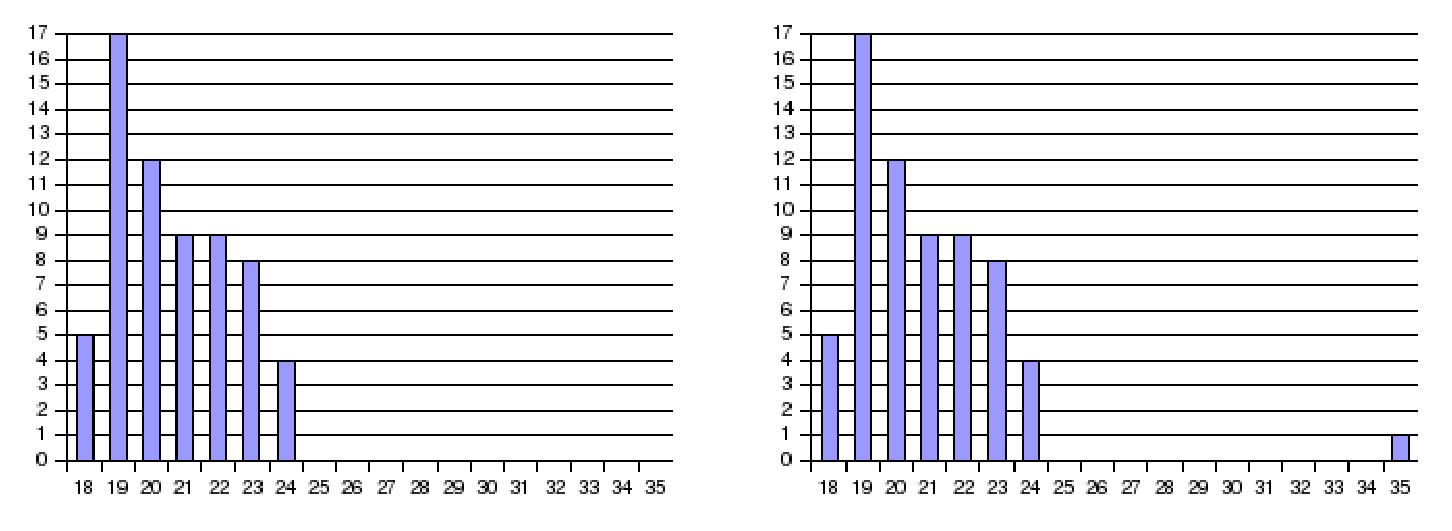
\includegraphics[height=3.5cm]{Dbes0113.eps}
\begin{picture}(0,0)
\put(-250,-5){\vector(-1,0){20}} 
\put(-250,-5){\vector(1,0){20}}
\put(-220,-7){Rang=6}
\put(-250,-15){\vector(-1,0){8}} 
\put(-250,-15){\vector(1,0){8}}
\put(-220,-20){RIQ=3}
\put(-65,-5){\vector(-1,0){60}} 
\put(-65,-5){\vector(1,0){60}}
\put(-2,-7){Rang=17}
\put(-100,-15){\vector(-1,0){9}} 
\put(-100,-15){\vector(1,0){9}}
\put(-2,-20){RIQ=3}
\end{picture}
\end{center}
}

\frame{\frametitle{Mesures de dispersi\'o}
\begin{itemize}
\item  \textbf{Desviaci\'o t\'{\i}pica}: mesura la difer\`encia entre les dades i el seu valor mitj\`a
\[
 \sigma_X=\sqrt{Var_X}
\]
\item $Var_X$ \'es la vari\`ancia de les dades
\item \only<1>{Es compleix que:}\only<2>{C\`alcul de la vari\`ancia amb dates brutes}\only<3->{C\`alcul de la vari\`ancia amb la taula de freq\"u\`encies}
\only<1>{
\begin{itemize}
\item Menys del $75\%$ dels valors est\`an continguts en $(\bar{x}-2\sigma_X,\bar{x}+2\sigma_X).$
\item Menys del $89\%$ dels valors est\`an continguts en $(\bar{x}-3\sigma_X,\bar{x}+3\sigma_X).$
\item Menys del $93\%$ dels valors est\`an continguts en $(\bar{x}-3\sigma_X,\bar{x}+3\sigma_X).$
\end{itemize}}
\only<2>{
\begin{itemize}
\item[] 
\[
 \bar{x}=\dfrac{x_1+x_2+\ldots+x_n}n,\quad Var_X=\dfrac{x_1^2+x_2^2+\ldots+x_n^2}n-\bar{x}^2
\]
\end{itemize}
}
\only<3->{
\begin{itemize}
\item[] 
\[
 \bar{x}=\dfrac{x_1n_1+x_2n_2+\ldots+x_kn_k}n,\quad Var_X=\dfrac{x_1^2n_1+x_2^2n_2+\ldots+x_k^2n_k}n-\bar{x}^2
\]
\end{itemize}
}
\item<4-> Per a dades agrupades en intervals els valors de $x_i$ es substitueixen per les \textbf{marques de classe}
\item<4-> Per a dades procedents de una mostra es calcula la vari\`ancia mostral 
\[
 VarM_X=\dfrac{n}{n-1}VarP_X
\]
\end{itemize}
}

\frame{\frametitle{Mesures de dispersi\'o}
\begin{itemize}
\item  Exemple de desviaci\'o t\'{\i}pica i vari\`ancia
\end{itemize}
\begin{columns}
\begin{column}{0.05\textwidth}
\begin{tabular}{|c|}\hline
7\\ \hline
5\\ \hline
9\\ \hline
7\\ \hline
5\\ \hline
6\\ \hline
7\\ \hline
6\\ \hline
4\\ \hline
\end{tabular}
\end{column}
\begin{column}{0.55\textwidth}
\only<2->{
$
\begin{array}{l}
\bar{x}=\dfrac{7+5+\ldots+4}{9}=6.22\\ \\
Var_{X}=\dfrac{7^2+5^2+\ldots+4^2}{9}-(6.22)^2\\
\hspace{0.9cm}=1.98 \\ \\
\sigma_X=\sqrt{Var_x}=1.4
\end{array}
$}
\end{column}
\begin{column}{0.1\textwidth}
\begin{tabular}{|c|c|} \hline
4 & 1 \\ \hline
5 & 2 \\\hline
6 & 2 \\\hline
7 & 3 \\\hline
9 & 1 \\\hline
\end{tabular}
\end{column}
\begin{column}{0.45\textwidth}
\only<3->{$
\begin{array}{l}
\bar{x}=\dfrac{4*1+\ldots+9*1}{9}=6.22\\ \\
Var_{X}=\dfrac{4^2*1+\ldots+9^2*1}{9}\\
\hspace{0.9cm}-(6.22)^2=1.98 \\ \\
\sigma_X=\sqrt{Var_x}=1.4
\end{array}
$}
\end{column}
\end{columns}
}

\frame{\frametitle{Mesures de dispersi\'o}
\begin{itemize}
\item  Representaci\' gr\`afica de la dispersi\'o: \textbf{Diagrames de capsa}
\end{itemize}
\begin{center}
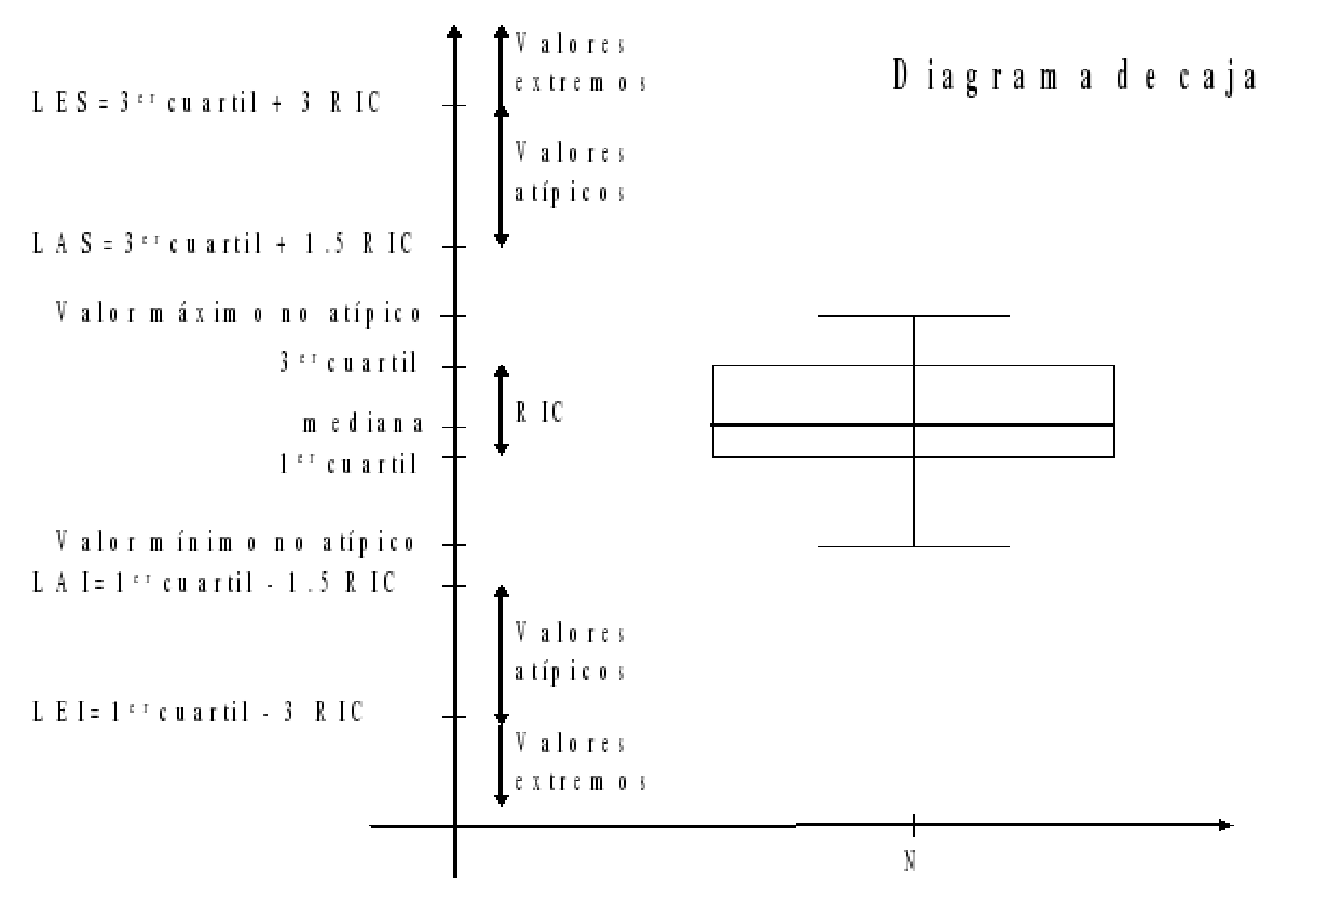
\includegraphics[height=7cm]{Dbes0114.eps}
\end{center}
}

\frame{\frametitle{Mesures de dispersi\'o}
\begin{itemize}
\item Exemple de diagrames de capsa
\end{itemize}
\usebeamerfont{child}
\begin{columns}
\begin{column}{0.3\textwidth}
\begin{tabular}{|c|c|c|} \hline
$x_i$ & $n_i$ &$ P_i$ \\ \hline
18&120  &19,1693  \\ \hline
19&150	&43,1310 \\ \hline
20&90	&57,5080 \\ \hline
21&70	&68,6901 \\ \hline
22&65	&79,0735 \\ \hline
23&50	&87,0607 \\ \hline
24&30	&91,8530 \\ \hline
25&20	&95,0479 \\ \hline
26&10	&96,6454 \\ \hline
27&7	&97,7636 \\ \hline
28&8	&99,0415 \\ \hline
29&2	&99,3610 \\ \hline
30&1	&99,5208 \\ \hline
34&1	&99,6805 \\ \hline
35&1	&99,8403 \\ \hline
40&1	&100,0000 \\ \hline
\end{tabular}
\usebeamerfont{normal}
\end{column}
\begin{column}{0.7\textwidth}
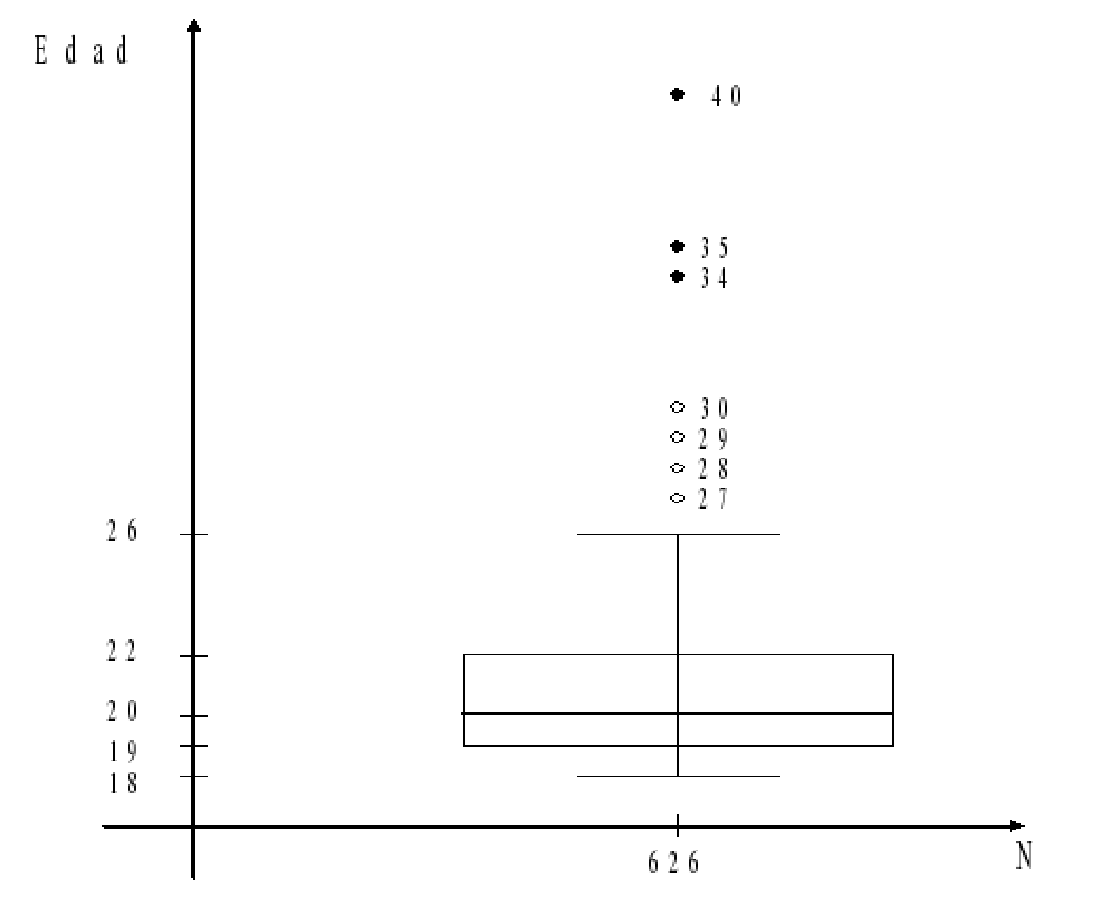
\includegraphics[height=5.5cm]{Dbes0115.eps} 
\end{column}
\end{columns}
\begin{picture}(0,0)
\put(5,-5){$n=626$}
\put(40,-5){$Q_1=19$}
\put(40,-17){$Q_3=22$}
\put(40,-29){mediana=20}
\put(80,-11){$RIC=3$}
\put(120,-5){$Q_1-1.5 RIC=14.5$}
\put(120,-17){$Q_3+1.5 RIC=26.5$}
\end{picture}
}

\frame{\frametitle{Mesures de dispersi\'o}
\begin{itemize}
\item Tipificaci\'o de dades estad\'{\i}stiques: z-scores
\begin{itemize}
\item La tipificaci\'o \'es un c\`alcul que permet comparar dades procedents de diferents estudis estad\'{\i}stics
\item Per a cada valor $x$ d'una variable estad\'{\i}stica (quantitativa) es calcula l'anomenat z-score
\[
 z=\dfrac {x-\bar{x}}{\sigma_X}
\]
\item Dues variables diferents es comparen comparant els seus respectius z-scores
\end{itemize}
\item <2->Dues persones opten a una beca esportiva. La primera t\'e una marca de 7.60m en salt de longitud i la segona una de 65.4s en 100 metres lliures de nataci\'o. Si tenim que en salt de longitud la mitjana \'es 7.40m i desviació típica \'es de 0.4m i en 100m lliures nataci\'o la mitjana \'es de 68.30s i la desviaci\'o t\'{\i}pica \'es de 1.6s, quina persona mereix més la beca? 
\item <3->
\[
z_1=\dfrac{7.60-7.40}{0.4}=0.5 \quad z_2=\dfrac{65.4-68.3}{1.6}=-1
\]
\end{itemize}
}

\end{document}